 The vertex  $\vec{A}$ can  be expressed  in {\em polar coordinate form} as
%\label{constr/tri/4/prob:tri_polar}
\begin{align}
\vec{A} &= c\myvec{\cos \theta\\  \sin \theta} ,\vec{B} = \myvec{0\\0},\vec{C} = \myvec{a\\0},
\\
\implies \vec{A} &= 5\myvec{\cos60 \\ \sin60} = \myvec{2.5 \\ 2.5\sqrt{3}} ,\vec{B} = \myvec{0\\0},\vec{C} = \myvec{6\\0}
\end{align}
upon substituting the given values.  The triangle is plotted in Fig.     \ref{constr/tri/4/fig:triangle LMN}.

\begin{figure}[ht]
    \centering
    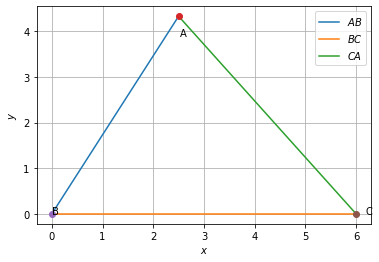
\includegraphics[width=\columnwidth]{solutions/triangle/4/assignment1 (2)/Figure1.png}
    \caption{$\triangle ABC$}
    \label{constr/tri/4/fig:triangle LMN}
\end{figure}

 
 
 

